% !TeX spellcheck = en_US
\documentclass[french]{yLectureNote}

\title{Optique ondulatoire - Méthodologie}
\subtitle{Physique}
\author{Paulhenry Saux}
\date{\today}
\yLanguage{Français}

\professor{B.Chalopin}
\usepackage{graphicx}%----pour mettre des images
\usepackage[utf8]{inputenc}%---encodage
\usepackage{geometry}%---pour modifier les tailles et mettre a4paper
%\usepackage{awesomebox}%---pour les boites d'exercices, de pbq et de croquis ---d\'esactiv\'e pour les TP de PC
\usepackage{tikz}%---pour deiffner + d\'ependance de chemfig
% \usepackage{tabularx}%---pour dimensionner automatiquement les tableaux avec variable X
\usepackage{awesomebox}%---Pour les boites info, danger et autres
\usepackage{menukeys}%---Pour deiffner les touches de Calculatrice
\usepackage{fancyhdr}%---pour les en-t\^ete personnalis\'ees
\usepackage{blindtext}%---pour les liens
\usepackage{hyperref}%---pour les liens (\`a mettre en dernier)
\usepackage{caption}%---pour la francisation de la l\'egende table vers Tableau
\usepackage{pifont}
\usepackage{array}%---pour les tableaux
\usepackage{lipsum}
\usepackage{yFlatTable}
\usepackage{multicol}
\newcommand{\Lim}[1]{\lim\limits_{\substack{#1}}\:}
\renewcommand{\vec}{\overrightarrow}
\newcommand{\N}[0]{\mathbb{N}}
\newcommand{\dd}{\mathrm{d}}
\newcommand{\norm}[1]{||\vec{#1}||}
\newcommand{\fo}{\psi(\vec{r},t)}
\newcommand{\foe}{\psi(\vec{r},t)\*}
\newcommand{\HH}{\hat{H}}
\newcommand{\hb}{\hbar}
\newcommand{\lap}{\nabla^2}
\newcommand{\lapcc}{\frac{\partial^2 }{\partial x^2}+\frac{\partial^2 }{\partial y^2}+\frac{\partial^2 }{\partial z^2}}
\newcommand{\mpsi}{\(\psi\)}
\newcommand{\und}{\underline}
\begin{document}
%Voir les notes de cours  à synthétiser
% Les rayons se propagent en ligne droite, sous les hypothèses :
% \begin{itemize}
%  \item milieu homogène
%  \item Diffraction négligée
%  \item Pas d'intéraction des rayons lumineux
% \end{itemize}
% Elles ont permis l'étude de la formtion d'image. L'Optique ondulatoire vise à comprendre les phénonèmes ondulatoires\marginCheck{Valable aussi pour d'autres ondes (son, onde gravitationnelle)}.
\chapter{Modèle scalaire}
\section{Étude de base}
\subsection{Trouver l'amplitude et \(\varphi\)}
L'onde étudiée est de la forme \(\und{\fo} = f(\vec{r})e^{-i(\omega t-\varphi(\vec{r}))}\).
\subsubsection{OPPM}
On suppose une OPPM se propageant dans la direction \(\vec{e_x}+\vec{e_y}\).

Comme on se trouve face à une OPPM, on sait que \(f(\vec{r}) = F_0 = \) Constante. On sait également que \(\varphi(\vec{r} = \vec{k}\cdot \vec{r})\) avec \(\vec{k}\) dans la direction de propagation de l'onde.

On ne va pas s'occuper de la norme de \(\vec{k}\). Trouvons le vecteur unitaire pointant dans sa ditection de propagation. On a donc :
\begin{flalign*}
\vec{k} &= k \frac{\vec{e_x}+\vec{e_y}}{||\vec{e_x}+\vec{e_y}||}\\
&= k \frac{\vec{e_x}+\vec{e_y}}{\sqrt{1^2+1^2}}\\
&= \frac{k}{\sqrt{2}} (\vec{e_x}+\vec{e_y})\\
\end{flalign*}
Il n'y a plus qu'à faire le produit scalaire manquant pour trouver l'expression finale :
\begin{flalign*}
\vec{k}\cdot \vec{r} &= \frac{k}{\sqrt{2}} (\vec{e_x}+\vec{e_y}) \cdot \vec{r}\\
&= \frac{k}{\sqrt{2}} (\vec{e_x}+\vec{e_y}) \cdot (x\vec{e_x}+y\vec{e_y})\\
&= \frac{k}{\sqrt{2}} (x+y)\\
\end{flalign*}
L'expression finale de l'onde est donc \[f_0 e^{-i(\omega t-(\frac{k}{\sqrt{2}} (x+y)))}\]
\subsubsection{Onde sphérique}
D'après le cours, on sait que \(f(\vec{r}) = \frac{A_0}{\norm{r_A}}\) avec \(\vec{r_A}\) le vecteur partant du centre de propagation de l'onde.

Ici, le centre est aux coordonnées \(-1,0,0\). On peut écrire \(\vec{r_A} = \vec{r}-\vec{r_o}\) avec \(\vec{r}(x,y,z)\) le vecteur partant de l'origine du repère jusqu'à une position étudiée et \(\vec{r_o}(-1,0,0)\) le vecteur partant de l'origine jusqu'au centre de propagation. On a donc \begin{flalign*}
\norm{r_A} &= ((x-(x_o)^2)+(y-(y_o)^2)+(z-(z_o)^2))^{\frac12}\\
&= ((x+1)^2+y^2+z^2)^{\frac12}
\end{flalign*}
\section{Appliquer des transformations}
On peut appliquer des contraintes aux ondes pour voir comment leur expression évoluent. Cela peut \^etre des miroirs ou des lentilles.
\subsection{Miroir}
\subsubsection{Exemples}

On reprend l'onde plane trouvée précédement, applique simplement les lois d'optique géométrique : la lumière est réflechit avec le m\^eme angle d'incidence par rapport à la normale du miroir.

Ainsi, pour une onde de vecteur d'onde de direction \(\vec{e_x}+\vec{e_y}\) se réfléchissant sur un miroir dans le plan \(O_yz\), la nouvelle direction sera \(-\vec{e_x}+\vec{e_y}\).

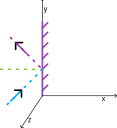
\includegraphics[scale=0.3]{methode-1}

Pour une onde sphérique, on prend simplement comme nouveau point de diffusion le symétrique du point original par rapport au miroir. Ainsi, pour une onde de source \(-1,0,0\) se réflechissant sur un miroir dans le plan \(Oxz\), l'onde réfléchhit est celle qui serait émise du point \((1,0,0)\)


\includegraphics[scale=0.5]{METHODE-2}
\subsubsection{Généralisation}
\includegraphics[scale=0.5]{methode-3}

De façon générale, pour une onde se propageant dans une dirction faisant un angle \(\alpha\) avec l'axe \(x\), le vecteur d'onde s'écrit \(\vec{k} = k\vec{u}\), avec
\begin{flalign*}
\vec{u} &= \frac{\cos(\alpha)\vec{e_x} + \sin(\alpha)\vec{e_y}}{||\cos(\alpha)\vec{e_x} + \sin(\alpha)\vec{e_y}||}\\
&= \frac{\cos(\alpha)\vec{e_x} + \sin(\alpha)\vec{e_y}}{\cos(\alpha)^2+\sin(\alpha)^2}\\
&= \cos(\alpha)\vec{e_x} + \sin(\alpha)\vec{e_y}
\end{flalign*}

Imaginons maintenant que le miroir fasse un angle \(\beta\) avec l'axe x\marginWarning{On image aussi que l'onde provient d'une source à l'infini, avec des ondes parallèles entre-elles.}. On ouhaite trouver la nouvelle expression du vceteur d'onde une fois l'onde réfléchie.

On peut remarquer immédiatement que pour que la réflexion ait lieu, il faut que \(\beta >\alpha\).

Si on utilise les angles avec la normale, l'angle d'incidence est \(\theta_i​=\alpha-\beta\). L'angle de réflexion est alors \(\theta_r​=-(\alpha-\beta)\) pour la réflexion.

Ainsi, l'angle que fait le vecteur d'onde réfléchi avec l'axe des x\marginInfo{La loi de la réflexion stipule que l'angle d'incidence est égal à l'angle de réflexion.} est \(\beta+(\beta-\alpha)=2\beta-\alpha\).

L'expression du vecteur d'onde réfléchi est donc :
$$ \vec{k}' = k \begin{pmatrix} \cos(2\beta - \alpha) \\ \sin(2\beta - \alpha) \end{pmatrix} $$

On peut vérifier que notre résultat est cohérent avec l'exemple précédent : On a \(\alpha = \frac{\pi}{4}, \beta = \frac{\pi}{2}\).

On a bien \(\cos(\pi-\frac{\pi}{4}) = -\frac{1}{\sqrt{2}}\) et \(\sin(\pi-\frac{\pi}{4}) = \sin(\frac{\pi}{4}) = \frac{1}{\sqrt{2}}\), ce qui correspond aux espressions trouvées.
\subsection{Lentille convergente}
On étudie maintenant une lentille convergente placée dans le plan \(Oyz\) de foyer image (1,0,0)
\subsubsection{Exemple}
On reprend l'onde de l'exemple de la section précédente. Il s'agit d'une onde plane. Elle va donc \^etre réfractée en une onde sphérique de centre le foyer image secondaire de la lentille\marginInfo{Cela serait le foyer image normal si l'onde plane était orthogonale à la lentille, mais ce n'est pas le cas car \(\vec{k} = \vec{e_x}+\vec{e_y}\)}. Schmétiquement, on voit que le foyer secondaire est à (1,1,0)

La nouvelle fonction s'écrit alors \[\fo = \frac{A_0}{r}e^{-i(\omega t -kr)}\] avec \(r = \sqrt{(x-1)^2+(y-1)^2+z^2}\).

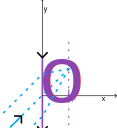
\includegraphics[scale=0.5]{lentille-1}
\subsubsection{Généralisation}
Pour une one plane dont le vecteur d'onde forme un angle \(a\) avec l'axe des x, on peut trouver le foyer secondaires avec la relation \(\tan(a) = \frac{H}{F_0} \Rightarrow H = F_0 \tan(a) \). Il ne reste alors plus qu'à remplacer la coordonné y dans la formule donnée en exemple.

\includegraphics[scale=0.5]{lentille-2}
\subsubsection{Onde sphérique centré sur le foyer objet}
L'objet sera alors à l'infini et les rayons seront orthogonaux à la lentille. Ici, l'onde sera alors une onde plane de la forme \[A_0 e^{-i(\omega t - \vec{k}\cdot \vec{r})} = A_0 e^{-i(\omega t - kx)}\]

\section{Calculer des chemins optiques}
Il s'agit de calculer la phase en un point de l'espace une fois que l'onde à parcouru certains milieux.

On sait que \(\varphi = k\times (AB)\), avec AB le chemin optique, qui dépend de \(n\) l'indice optique.

On peut écrire :
\begin{flalign*}
\varphi_B &= k \times (AB)\\
&= \frac{2\pi}{\lambda_0} \times \int_A^B n(l)\dd l\\
\end{flalign*}
On peut ensuite couper l'intégrale en plusieurs parties à chaque fois que l'indice optique change.
\checkInfo{Exemple}{
Imaginons un rayon traversan une cuve de longueur intérieure $d$ et d'épasseur $e$ faite en verre (\(n_v = 1.5\)) et remplie d'eau (\(n_e = \frac{4}{3}\)). La phase de l'onde à l'arrivée est donc de
\begin{flalign*}
\varphi_B &= k \times (AB)\\
&= \frac{2\pi}{\lambda_0} \times \int_A^B n(l)\dd l\\
&= \frac{2\pi}{\lambda_0} \times (\int_0^e n_v\dd l + \int_e^d n_e\dd l + \int_d^e n_v\dd l)\\
&= \frac{2\pi}{\lambda_0}(2e\cdot n_v + d\cdot \frac{4}{3})
\end{flalign*}
}
\section{Analyse de graphique}
\includegraphics[scale=0.2]{graph}

On considère une onde plane monochromatique dont la fonction d’onde est représentée en bleue
en fonction de l’axe des x horizontal gradué en m, à t = 0 en train plein, et à t = 1 s en pointillés en violet. On cherche à trouver ses propriétés.

La longueur d'onde est de 0.5m car l'onde se répète tous les 0.5m.

On ne peut pas déterminer une valeur de vitesse, mais on peut donner des valeurs possibles.

La vitesse est \(\frac{\Delta x}{\Delta t}\). Ici, \(\Delta t = 1s\), mais \(\Delta x\) reste indéterminée. En effet, il peut \^etre de \(-0.1\)m, de \(+0.4\)m. En fait \(\Delta x = 0.4[\lambda]\). On en déduit que \[v = \frac{0.4+n\lambda}{1} = 0.4+n\cdot \lambda\] avec \(n\in \N\).

En supposant maintenant que \(v = 0.5m/s\), on cherche à trouver la pulsation de l'onde. On sait que \(\omega  = \frac{2\pi}{T}\) et que \(\lambda = v T\), donc \[\omega = \frac{2\pi v}{\lambda}\]

La fonction s'écrit donc \[\fo = A\cos(kx-\omega t+\varphi_0)\]. La phase à l'orgine (temporelle et spatiale ) est de 1, donc on peut choisir \(\varphi_0 = 0\). En notation complexe, on peut écrire \[\fo = A_0e^{-i(\omega t-kx)}\]
\section{Utiliser des fonctions d'onde}
\subsection{Équation d'onde}
On considère la fonction d'onde :
$$ψ(\vec{r}, t) = ψ(y, t) = Ae^{-(\alpha y + \beta t)^2}$$
Pour que cette fonction soit solution de l'équation d'onde 1D, elle doit vérifier :
$$ \frac{1}{v^2} \frac{\partial^2 ψ}{\partial t^2} = \frac{\partial^2 ψ}{\partial y^2} $$

Calculons la dérivée partielle par rapport à t.

\begin{flalign*}
\frac{\partial \psi}{\partial t} &= A \cdot e^{-(\alpha y + \beta t)^2} \cdot \frac{\partial}{\partial t}(-(\alpha y + \beta t)^2)\\
&= Ae^{-(\alpha y + \beta t)^2} \cdot (-2(\alpha y + \beta t) \cdot \beta)\\
&= -2A\beta(\alpha y + \beta t)e^{-(\alpha y + \beta t)^2}
\end{flalign*}
On peut maintenant effectuer la dérivée seconde, en utilisant la règle du produit $(uv)' = u'v + uv'$ :

\begin{flalign*}
\frac{\partial^2 \psi}{\partial t^2} &= -2A\beta \left[ \frac{\partial}{\partial t}(\alpha y + \beta t) \cdot e^{-(\alpha y + \beta t)^2} + (\alpha y + \beta t) \cdot \frac{\partial}{\partial t}(e^{-(\alpha y + \beta t)^2}) \right]\\
&= -2A\beta \left[ \beta e^{-(\alpha y + \beta t)^2} + (\alpha y + \beta t) \cdot (-2\beta(\alpha y + \beta t)e^{-(\alpha y + \beta t)^2}) \right]\\
&= -2A\beta^2 e^{-(\alpha y + \beta t)^2} + 4A\beta^2 (\alpha y + \beta t)^2 e^{-(\alpha y + \beta t)^2}\\
&=2A\beta^2 e^{-(\alpha y + \beta t)^2} \left[ 2(\alpha y + \beta t)^2 - 1 \right]
\end{flalign*}

On calcule maintenant la dérivée partielle par rapport à y :
\begin{flalign*}
\frac{\partial \psi}{\partial y} &= A \cdot e^{-(\alpha y + \beta t)^2} \cdot \frac{\partial}{\partial y}(-(\alpha y + \beta t)^2)\\
&= Ae^{-(\alpha y + \beta t)^2} \cdot (-2(\alpha y + \beta t) \cdot \alpha)\\
&= -2A\alpha(\alpha y + \beta t)e^{-(\alpha y + \beta t)^2}
\end{flalign*}
puis la dérivée seconde :
\begin{flalign*}
\frac{\partial^2 \psi}{\partial y^2} &=
-2A\alpha \left[ \frac{\partial}{\partial y}(\alpha y + \beta t) \cdot e^{-(\alpha y + \beta t)^2} + (\alpha y + \beta t) \cdot \frac{\partial}{\partial y}(e^{-(\alpha y + \beta t)^2}) \right]\\
&= -2A\alpha \left[ \alpha e^{-(\alpha y + \beta t)^2} + (\alpha y + \beta t) \cdot (-2\alpha(\alpha y + \beta t)e^{-(\alpha y + \beta t)^2}) \right]\\
&= -2A\alpha^2 e^{-(\alpha y + \beta t)^2} + 4A\alpha^2 (\alpha y + \beta t)^2 e^{-(\alpha y + \beta t)^2}\\
&=\frac{\partial^2 ψ}{\partial y^2} = 2A\alpha^2 e^{-(\alpha y + \beta t)^2} \left[ 2(\alpha y + \beta t)^2 - 1 \right]
\end{flalign*}

\subsection*{Vérification de l'équation d'onde}

On substitue les dérivées dans l'équation d'onde :
$$
\frac{1}{v^2} \left( 2A\beta^2 e^{-(\alpha y + \beta t)^2} \left[ 2(\alpha y + \beta t)^2 - 1 \right] \right) = 2A\alpha^2 e^{-(\alpha y + \beta t)^2} \left[ 2(\alpha y + \beta t)^2 - 1 \right]
$$
En simplifiant les termes communs :
$$
\frac{\beta^2}{v^2} = \alpha^2 \Rightarrow v^2 = \frac{\beta^2}{\alpha^2} \Rightarrow v = \pm \frac{\beta}{\alpha}$$

La fonction est bien solution de l'équation d'onde si la vitesse est $v = \frac{\beta}{\alpha}$ dans le sens des y négatifs.
\subsection{Fonction d'onde}
On considère une onde progressive se propageant dans la direction des z croissants à la vitesse
v = 2 m/s et dont la fonction d’onde à t = 0 s’écrit :\[\psi(z,t=0) = \frac{C}{1+z^2}\]
avec C une constante. On veut donner l’expression de la fonction d’onde pour z et t quelconques et représenter cette fonction en fonction du temps pour z = 0 et z = 1 m.

L'onde se propage dans la direction des $z$ croissants. L'expression générale est de la forme $\psi(z, t) = f(z-vt)$.
Par identification, on a $f(z) = \frac{C}{1+z^2}$.
En remplaçant l'argument $z$ par $z-vt$, on obtient l'expression de la fonction d'onde à un instant $t$ quelconque :
$$ \psi(z, t) = \frac{C}{1+(z-vt)^2} $$
Avec la vitesse $v = 2$ m/s :
$$ \psi(z, t) = \frac{C}{1+(z-2t)^2} $$

\subsection*{Représentation en fonction du temps}

\subsubsection*{Pour $z=0$}
$$
\psi(0, t) = \frac{C}{1+(0-2t)^2} = \frac{C}{1+4t^2}
$$
Cette fonction est une courbe de Lorentz centrée sur $t=0$, avec un maximum $\psi(0,0)=C$.

\subsubsection*{Pour $z=1$ m}
$$
\psi(1, t) = \frac{C}{1+(1-2t)^2}
$$
Cette fonction est également une courbe de Lorentz. Le maximum de l'onde se produit lorsque l'argument du dénominateur est nul, c'est-à-dire quand $1-2t=0$. Le pic de l'onde se situe à $t=0,5$ s, ce qui correspond au temps de propagation de l'onde sur une distance de 1 m à la vitesse de 2 m/s. La forme de la courbe est la même, mais décalée dans le temps.

On peut les représenter :

\includegraphics[scale=0.2]{graph2}

 \end{document}
